\chapter{Enzymes: The Right Reaction at the Right Time}

\begin{kaichang}
\textbf{Translator safety note:} Follow the tenderizer label and keep raw meat refrigerated during holding or marinating, rather than adopting the room-temperature example as a food-safety rule. Prevent cross-contamination and cook to an appropriate measured internal temperature. See \href{https://www.fsis.usda.gov/food-safety/safe-food-handling-and-preparation/food-safety-basics/steps-keep-food-safe}{USDA food-safety guidance}.

In the supermarket seasoning aisle is a white powder called ``meat tenderizer.'' Its instructions seem almost suspiciously simple: sprinkle a little over tough raw beef, mix, and leave at room temperature for half an hour---no heating, no vinegar, nothing else. Cook it afterward, and the once-unchewable meat becomes smooth and tender.

Guess what the powder did. Did it ``soak the meat soft,'' secretly heat it, or contain something that ``bites'' the meat? Read the small print: the main ingredient is ``papain,'' with a warning not to mix it with boiling water. Why does it fear boiling water?

Place your bet on paper. We will reveal the answer at the chapter's end. This unassuming powder will take us across one of the book's most important boundaries: from the chemistry of matter into the chemistry of life.
\end{kaichang}

\section{Three Kitchen Puzzles}

\textbf{Translator safety note:} The peroxide description below is not wound-care advice. Hydrogen peroxide is no longer recommended for wound disinfection because it can damage healing cells. Do not reproduce the example on skin; see \href{https://www.poison.org/articles/hydrogen-peroxide}{Poison Control's guidance}.

Tenderizer is not the only puzzle. Here are two more, both things I can practically guarantee you have encountered.

First: put bland, unsweetened steamed wheat bread in your mouth and chew slowly without rushing to swallow. After a minute, a distinct sweetness emerges. Yet its ingredient list contains no sugar.

Second: hydrogen peroxide used on wounds can sit in its bottle for years with little visible change, but one small drop on cut raw pig liver or potato immediately releases abundant bubbles as though boiling. They are oxygen. No heat, no electricity, just contact with a little liver.

Third: ordinary soap struggles with milk and blood stains, but soaking clothes in ``enzyme detergent'' cleans them. Yet its label recommends warm water around $40\,^{\circ}\mathrm{C}$, not scalding water.

These puzzles seem unrelated: meat, bread, peroxide, and clothes. Put them together, however, and common features emerge:

\begin{itemize}[itemsep=2pt]
\item Changes occur under \textbf{mild conditions}: ordinary temperature and pressure, without strong acids or bases;
\item Only \textbf{tiny amounts of a mysterious ingredient} are needed: a spoonful of powder, a mouthful of saliva, a drop of liver juice;
\item Each ingredient \textbf{handles only one job}: tenderizer does not break down milk stains, and saliva does not make peroxide bubble;
\item They all \textbf{dislike heat}.
\end{itemize}

Chemists over a century ago were puzzled by the same things. They could catalyze reactions in flasks with platinum, iron, or sulfuric acid (Chapter 30), but laboratory catalysts either required high temperatures and pressures or ``catalyzed everything without precision.'' Biological ingredients were remarkably specific, efficient, and mild. They became known collectively as \textbf{enzymes}---catalysts made by living organisms.

\section{Zooming In: A Folded Pocket}

Chapter 48 explained that proteins are amino-acid chains folded into three-dimensional structures, with folding determining function. Enzymes are proteins specialized in folding a ``workshop.''

The workshop is the \textbf{active site}, a distinctively shaped small pocket or groove usually occupying only a tiny part of the surface. A few selected amino-acid side chains line it: positive, negative, hydrophobic, or hydrogen-bonding---all Chapter 48's temperaments put to work. A molecule admitted to this pocket and reacting there is the enzyme's \textbf{substrate}.

Substrates collide randomly in solution. One entering an active site with matching shape and charge is caught: hydrogen bonds, electrostatic attraction, and hydrophobic interactions hold it in a particular orientation and position. This temporary association is the \textbf{enzyme--substrate complex}. Side chains then act: one pulls a substrate bond, another passes a proton, another temporarily accepts an electron pair. After reaction, the products no longer fit and leave. The enzyme returns to its original state, awaiting another substrate.

German chemist Fischer first described this specificity in 1894---the Fischer mentioned for esterification in Chapter 40. He proposed a \textbf{lock-and-key} relationship: a fixed keyhole admits only a fitting key. This explains specificity: salivary amylase's lock recognizes starch, not the peroxide key.

But the model has a flaw. If the lock cannot change shape at all, how can it fit both the entering substrate and its different shape during reaction? In 1958, American scientist Koshland proposed the more realistic \textbf{induced fit}: an active site resembles not a rigid lock but a \textbf{glove}. Empty, it lies flat; a hand entering stretches it into a close fit. Likewise, substrate entry slightly adjusts the pocket, wrapping it more tightly and squeezing it into a favorable reactive pose: lengthening the necessary bond, bringing groups together, and excluding water where needed.

An enzyme therefore does more than recognize its substrate: it \textbf{actively changes the substrate's circumstances}. That action is the next section's subject.

\section{What Enzymes Do: Lower the Mountain}

Recall Chapter 29: even an energy-releasing reaction that ``wants'' to happen must cross an \textbf{activation-energy} mountain. Reactants must bend, stretch, and approach an awkward transition state before descending to products. Higher mountains admit fewer molecules and slow reactions. Chapter 30 explained the catalyst's general strategy: not pushing molecules, but \textbf{building a tunnel}, providing another pathway with lower activation energy.

Enzymes do exactly this with extraordinary craftsmanship. Induced fit supports the transition state: the substrate approaches its geometry, while the pocket's charges stabilize its developing charges, cutting a substantial height from the peak.

This is the chapter's most important diagram to remember. It is a human-made representation; horizontal ``reaction progress'' is not a real distance.

\begin{center}
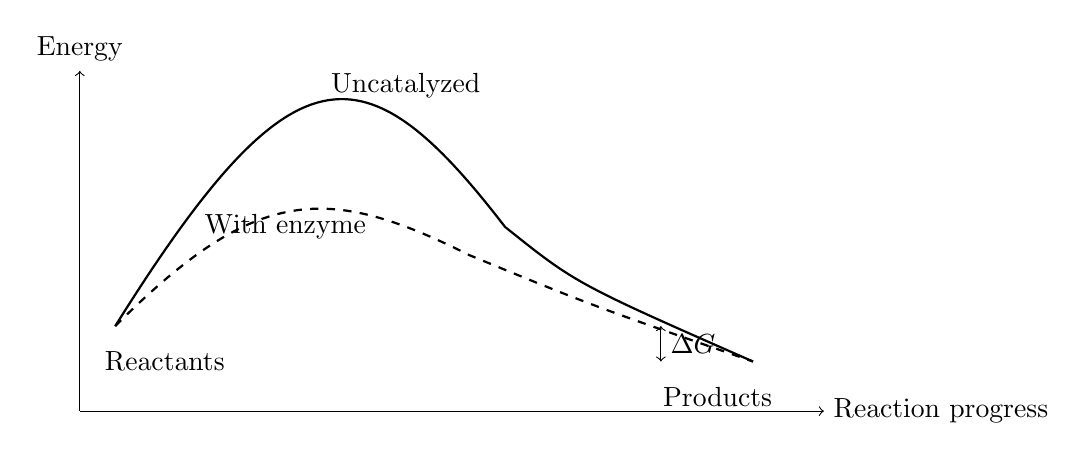
\begin{tikzpicture}[scale=0.9]
\draw[->] (0,0) -- (10.5,0) node[right]{Reaction progress};
\draw[->] (0,0) -- (0,4.8) node[above]{Energy};
\draw[thick] (0.5,1.2) .. controls (3,5.2) and (4,5.2) .. (6,2.6)
   .. controls (7,1.8) .. (9.5,0.7);
\draw[thick,dashed] (0.5,1.2) .. controls (2.5,3.2) and (3.5,3.2) .. (5.5,2.2)
   .. controls (7.2,1.5) .. (9.5,0.7);
\node at (1.2,0.7) {Reactants};
\node at (9,0.2) {Products};
\node at (4.6,4.6) {Uncatalyzed};
\node at (2.9,2.6) {With enzyme};
\draw[<->] (8.2,0.7) -- (8.2,1.2) node[midway,right]{$\Delta G$};
\end{tikzpicture}
\end{center}

The solid curve is the mountain without enzyme; the dashed curve is the lower route with it. Notice two things. First, \textbf{the starting and finishing heights do not change}. The reactant--product free-energy difference $\Delta G$ belongs to the molecules themselves (Chapter 28); the enzyme has not touched it. Second, this implies a frequently troublesome conclusion: \textbf{enzymes do not change equilibrium}. Chapter 31 assigned equilibrium position to $\Delta G$. With it unchanged, the eventual reactant and product proportions are identical with or without enzyme. Enzymes simply get you there \textbf{faster}. By lowering activation energies in both directions, they accelerate both without favoritism.

Remember three things enzymes do not do: \textbf{supply energy} (they lower the mountain, not push molecules); \textbf{change direction} (no amount of enzyme makes an originally unwilling, positive-$\Delta G$ reaction occur); or \textbf{change the endpoint} (equilibrium stays fixed). We will use these repeatedly.

How much lower is the mountain? Get a numerical feel for it.

\begin{qiaoliang}
Consider hydrogen peroxide, \chem{H_2O_2}, decomposing into water and oxygen. Uncatalyzed, it is slow enough for a bottle to last years. Liver's \textbf{catalase} makes the route nearly level: \textbf{one} molecule decomposes about $10^{5}$ to $10^{6}$ peroxide molecules per second, among nature's fastest enzymes. A drop of ground-liver extract contains roughly $10^{15}$ enzyme molecules, together able to handle about $10^{20}$ peroxide molecules per second. How many molecules are in a drop of $3\%$ peroxide? About $10^{19}$. Thus one drop of liver juice could theoretically clear one drop of peroxide in \textbf{less than a second}, explaining the ``instant boiling'' of bubbles. Without enzymes, the same molecules must slowly climb by chance for years. The same mountain, with or without a tunnel, differs in time by roughly $10^{8}$-fold. Many enzymatic accelerations range from $10^{5}$ to $10^{17}$. Without enzymes, most bodily reactions would be so slow as to be practically absent, making life chemically impossible.
\end{qiaoliang}

\section{Symbols: \texorpdfstring{$\chem{E}$ Plus $\chem{S}$}{E Plus S}}

With the rules clear, symbols can appear. The general scheme is:

\[\chem{E} + \chem{S} \rightleftharpoons \chem{ES} \rightarrow \chem{E} + \chem{P}\]

$\chem{E}$ is enzyme, $\chem{S}$ substrate, $\chem{ES}$ the enzyme--substrate complex, and $\chem{P}$ product. The enzyme enters on the left and emerges unchanged on the right. Like every catalyst in Chapter 30, it \textbf{is not consumed}. Hence a spoonful of tenderizer handles a large piece of meat: every enzyme can take thousands of repeat orders.

The reaction making bread sweet in saliva is starch hydrolysis (Chapter 46 discussed carbohydrates and glycosidic bonds):

\[\chem{(C_6H_{10}O_5)_{n}} + n\chem{H_2O} \rightarrow n\chem{C_6H_{12}O_6}\]

Salivary amylase cuts starch chains into sections, first producing shorter dextrins and maltose. The sweetness comes from released small sugars. Without the enzyme, that same bread would have to soak in your stomach for an unknown length of time before becoming useful.

Another symbolic rule deserves attention: rate versus substrate concentration. Fix enzyme amount and increase substrate. Rate initially rises almost proportionally, then flattens progressively toward a horizontal limit. Why? At low concentration, many pockets are empty, so more substrate means more working pockets. Eventually all pockets are \textbf{occupied around the clock}; enzymes cannot keep up even working continuously, and extra substrate must queue. Rate reaches its ceiling, $V_{\max}$, the maximum rate. The substrate concentration at half $V_{\max}$ is $K_{\mathrm{m}}$, the Michaelis constant, roughly an index of pocket--substrate affinity: smaller $K_{\mathrm{m}}$ means less substrate is needed for half-saturation and tighter capture.

\begin{shiyan}
Test that your saliva contains enzymes, safely at home. Materials: a small piece of steamed wheat bread or a spoonful of rice, two clean small dishes, pharmacy povidone-iodine (iodine solution), warm water, and clean chopsticks. Steps: (1) Tear the bread into two similar portions. (2) Chew one thoroughly for a minute, saturating it with saliva, then spit it onto a dish; use only your own saliva, without sharing. (3) Add an equal amount of warm water to the other portion and mash it similarly. (4) Add one iodine drop to each and compare colors. Chapter 46 explained that starch turns deep blue with iodine. The water-treated portion should turn distinctly blue; the chewed one should be much paler or uncolored because amylase has cut some starch. Safety note: iodine is external-use only and must never enter your mouth; wash hands afterward. Keep saliva-contact utensils for your own use and clean them. For a clearer comparison, hold both samples in a warm-water bath around $37\,^{\circ}\mathrm{C}$ for five minutes before adding iodine. Think about why near-body temperature works best.
\end{shiyan}

\section{How Scientists Know: Enzymes Are Not a Vital Force}

\begin{zhengju}
In the nineteenth century, brewing and breadmaking were ancient crafts, yet fermentation's nature remained disputed for decades. Pasteur's school insisted on \textbf{living} yeast: a ``vital force'' exclusive to living cells turned sugar into alcohol, beyond chemistry alone. It sounded plausible: boil yeast dead, and fermentation stops.

In 1897, German chemist Eduard Buchner intended to use pressed yeast juice for medical research. Adding sugar as a preservative unexpectedly produced bubbles: cell-free juice fermented sugar into alcohol. \textbf{Fermentation occurred without living cells}. The supposed vital force was a group of substances inside yeast---enzymes---capable of working independently outside cells. His design was delightfully simple: living cells versus cell-free juice, changing one variable while holding others constant. Microscopy and repeated dilution excluded the alternative of residual intact cells. This bubbling jar reclaimed life's chemistry from mysticism for chemistry.

Next came the question of what enzymes were. In 1926, American chemist Sumner purified urease from jack beans and \textbf{crystallized} it. Crystallization then signified a pure compound, and the crystals were protein. His declaration that ``enzymes are proteins'' met ridicule: authorities thought proteins too ``dirty,'' merely impurities adsorbing the true active ingredient. Debate lasted almost a decade, until successive enzyme crystals all proved to be proteins. Later discovery of a few catalytic RNAs, ribozymes, added a footnote to ``all enzymes are proteins.'' Evidence repeatedly forces scientific conclusions to accept patches.

How enzyme and substrate bind follows the earlier story: Fischer's 1894 lock-and-key model ruled for over half a century until Koshland's 1958 induced fit added a moving lock rather than overturning the model. Evidence supported the revision: X-ray crystallography later pictured the same enzyme with and without substrate, showing different shapes. From vital force to protein to changing pocket, each step was not a flash of genius but \textbf{a concession after experiments cornered an older explanation}.
\end{zhengju}

\section{Weak Points: Damage, Blockage, and Miscalculation}

Enzymes now seem almost perfect. Yet precisely because they depend on finely folded protein structure (Chapter 48), they have real weaknesses.

\textbf{First, heat can unravel them.} Rising temperature increases molecular motion and usually reaction rate, so enzymatic rate initially rises. Above a threshold, hydrogen bonds and hydrophobic interactions cannot maintain the fold: the protein denatures (Chapter 48), its pocket collapses, and it permanently stops working. Hence tenderizer and enzyme detergent dislike boiling water. Most human enzymes are most comfortable near body temperature, while hot-spring bacterial enzymes withstand above $70\,^{\circ}\mathrm{C}$. Optimum temperature depends on the source organism, not a universal standard.

\textbf{Second, pH matters.} Side-chain charges depend on environmental pH (Chapter 32), so pH changes pocket charge and shape. Stomach pepsin is most active around strongly acidic pH $2$ and falters in the small intestine's mildly alkaline conditions. Trypsin takes over, favoring pH about $8$. Along digestion, pH changes like a relay baton and successive enzymes change shifts.

\textbf{Third, enzymes can be blocked---the basis of many medicines.} If a pocket recognizes a substrate, a similar-shaped molecule unable to react normally can occupy it. This is \textbf{competitive inhibition}: inhibitor and substrate compete for the same seat, which sufficiently high substrate concentration can reclaim. Early sulfonamide antibiotics use this idea. Bacteria need an enzyme to make folate; sulfonamides resemble its substrate and occupy its seat without working, cutting folate supplies and stopping reproduction. Human cells obtain folate from food rather than synthesizing it, so largely avoid collateral damage. A good drug finds \textbf{an enemy's pocket that you lack}. A more complete blockage is aspirin (Chapter 44): it \textbf{permanently welds shut} the active site of cyclooxygenase by covalent binding. That enzyme molecule is finished, and pain relief fades only after the body makes new enzyme: irreversible inhibition. Another kind does not compete for the seat. Binding \textbf{outside} the pocket changes the whole protein and distorts the site, so arriving substrate cannot stay. This is \textbf{noncompetitive inhibition}, where extra substrate cannot restore rate. Many poisons, including certain heavy-metal ions, similarly deform key enzymes.

\textbf{Fourth, the elegant formula has limited conditions.} Michaelis and Menten expressed the rising-then-leveling rate pattern in 1913 in a concise equation (the closing challenge), successfully describing many enzymes. Its assumptions include measuring \textbf{initial} rate, before product accumulation or significant reverse reaction; far more substrate than enzyme; approximately constant enzyme--substrate complex concentration; and \textbf{one} substrate without regulation. Real cells often violate these: product feedback inhibition, remote regulation by other molecules, or substrates changing enzyme behavior through allostery like hemoglobin's. The equation is not wrong, but using it universally oversteps its model's boundaries.

\begin{wuqu}
``Drink enzyme supplements to replenish your body's enzymes, improve digestion, detoxify, and prevent aging.'' Popular products fail on two levels. First, enzymes are proteins: swallowed enzymes meet stomach acid and pepsin, a protein-dismantling machine, and are cut into small amino-acid pieces for absorption. They are \textbf{extremely unlikely} to enter blood intact and report for work. In this sense, drinking enzymes differs little from drinking egg-drop soup. Second, even an intact absorbed enzyme would not know which pocket to visit. Specificity restricts it to one reaction; no universal detoxifying enzyme exists. A qualification matters: some oral enzyme preparations do work, such as lactase taken with meals by lactose-intolerant people (Chapter 46). Its workplace is the gut itself; it breaks lactose locally without absorption. Effectiveness's boundary is always \textbf{mechanism}, not advertising. Whether you buy is your choice, but know which level your money pays for.
\end{wuqu}

\section{Back to the Tenderizer}

Now reveal the answer. Papain is a protein extracted from papaya latex. Sprinkled on meat, its active site recognizes long collagen and muscle-fiber proteins and cuts their peptide bonds (Chapter 48). Meat's toughness comes from these tangled long chains; shorter pieces naturally give a tenderer texture.

Check every opening puzzle:

\begin{itemize}[itemsep=2pt]
\item \textbf{Why does room temperature suffice?} Lower activation energy lets ordinary molecular thermal motion cross the smaller hill without heating.
\item \textbf{Why only a little?} Enzymes are not consumed; each takes thousands of repeat orders.
\item \textbf{Why avoid boiling water?} Heat denatures the protein, collapsing pocket and tunnel and turning tenderizer into ordinary protein powder.
\item \textbf{Why does it not tenderize other things?} Papain recognizes proteins, so you need not fear it corroding your plate.
\end{itemize}

The other puzzles follow: salivary amylase cuts bread's starch into small sugars near body temperature; liver catalase rapidly detoxifies peroxide into water and oxygen. Peroxide is toxic to cells, and you merely borrowed this enzyme's overtime work.

\section{Speed Is Not Enough: Who Decides Whether?}

Outside kitchens, enzymes form an industrial workforce. Detergents combine proteases, lipases, and amylases against blood/milk stains, oil, and food residue. Warm water provides optimum working conditions, explaining warm washing. Food manufacturers use glucose isomerase to turn some corn-syrup glucose into sweeter fructose, producing millions of tonnes of high-fructose syrup annually. Cheese depends on rennet cutting milk casein; biofuels need cellulases breaking tough plant-wall cellulose (Chapter 46). Many marketed medicines target enzymes; blocking a critical pocket is a central modern drug-design strategy.

But a closing caution also prepares the next chapter. Enzymes determine \textbf{speed}, not \textbf{direction}. Yet cells constantly assemble amino acids into protein, build larger molecules, and pump substances against concentration gradients, all energy-requiring. These have positive $\Delta G$ and are unwilling by Chapter 28's verdict, which no enzyme can alter.

How does life run these unwilling reactions every day without pause? Cells have an energy-transfer system \textbf{coupling} favorable energy-releasing reactions to unfavorable energy-requiring ones, letting the former pull the latter. Its common currency is the familiar ATP. How does energy transfer, and why is ``ATP contains high-energy bonds'' problematic? Chapter 50 will inspect the cellular ledger.

\begin{tiaozhan}
The Michaelis--Menten equation is (skipping this does not affect the main thread):

\[v = \frac{V_{\max}\,[\chem{S}]}{K_{\mathrm{m}} + [\chem{S}]}\]

Here $v$ is initial rate and $[\chem{S}]$ substrate concentration. Verify three limits: (1) When $[\chem{S}]$ greatly exceeds $K_{\mathrm{m}}$, the denominator is approximately $[\chem{S}]$, giving $v\approx V_{\max}$: full pockets and maximum rate. (2) When $[\chem{S}]=K_{\mathrm{m}}$, $v = V_{\max}/2$, the definition of $K_{\mathrm{m}}$. (3) When $[\chem{S}]$ is far below $K_{\mathrm{m}}$, $v\approx (V_{\max}/K_{\mathrm{m}})\,[\chem{S}]$: rate proportional to substrate, with many empty pockets. The equation follows from $\chem{E}+\chem{S}\rightleftharpoons\chem{ES}\rightarrow\chem{E}+\chem{P}$, assuming approximately constant $\chem{ES}$ early in the reaction, the steady-state assumption. Product inhibition of substrate, remote enzyme regulation, or significant reverse reaction requires rewriting it. A formula comes packaged with its assumptions; remembering this matters more than memorizing the formula itself.
\end{tiaozhan}

\section*{Exercises}

\begin{sikaoti}
\item Draw two energy diagrams for the same energy-releasing reaction, with and without enzyme. Mark activation-energy and $\Delta G$ arrows in each. Which changes with enzyme, and which does not? Explain why enzymes do not change equilibrium.
\item One catalase molecule decomposes about $10^{6}$ peroxide molecules per second. Treating a bottle of $3\%$ peroxide containing about $10^{22}$ molecules requires approximately $10^{16}$ enzyme molecules working together. A \ud{500}{g} liver has about $10^{11}$ cells, each assumed to contain $10^{7}$ catalase molecules. Estimate the total and whether it suffices, with how many times the requirement.
\item Bread dough proofs in a warm place, but enzymes stop working during steaming. Explain both stages with a temperature--rate curve that rises then falls, marking approximate proofing and steaming regions.
\item A competitive inhibitor resembles the substrate. Draw particles using notched circles for enzyme pockets, triangles for substrate, and squares for inhibitor, showing substrate alone, added inhibitor, and greatly increased substrate. Explain why extra substrate reverses competitive but not noncompetitive inhibition.
\item What happens if pepsin, optimal around pH $2$, and trypsin, optimal around pH $8$, exchange environments? Explain in terms of side-chain charges altering pocket shape, and discuss implications for oral enzyme supplements.
\item Someone claims a superenzyme converts $100\%$ of reactants into products. Refute this using each of the three things enzymes do not do. To increase equilibrium product proportion, what quantity should actually be changed? (Hint: Chapters 28 and 31.)
\end{sikaoti}
